\section{Project burndown chart}\label{sec:burndown}

The burndown chart for the entire project can be seen in figure \ref{fig:bdchart}. We estimated our velocity to be quite low for the first sprint since we figured it would take time to get acquainted with the project, the work environment and the tools we would need to work with. After that we estimated that our velocity would increase and average out to about 77 story points per sprint during the 12 week semester. For the last two sprints we estimated our velocity to be 114 story points per sprint as we would have more capacity during those sprints. 

We finished a total of 570 story points which gave us a velocity of 81.4 story points per sprint. Therefore our estimate was not far off the mark, although we sometimes did get behind schedule, we always managed to make up for it and we ultimately reached our goal. 
	
\begin{figure}[H]
  \centering
  \graphicspath{ {./graphics/} }
  \centerline{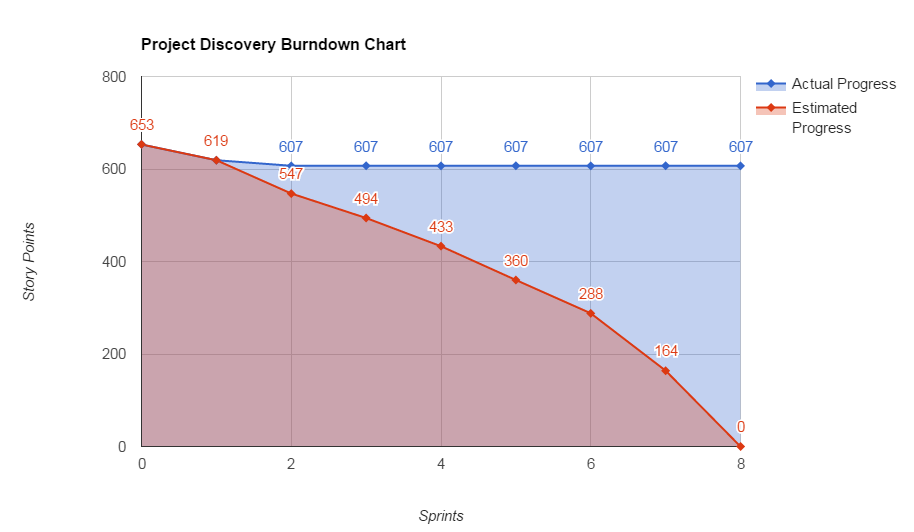
\includegraphics[scale=0.55]{bdchart.png}}
  \caption{\label{fig:bdchart} Burndown chart for the whole project.}
\end{figure}
